\documentclass[12px]{article}

\usepackage{tikz}
\usepackage{geometry}
\usetikzlibrary{mindmap}

\begin{document}
\begin{center}
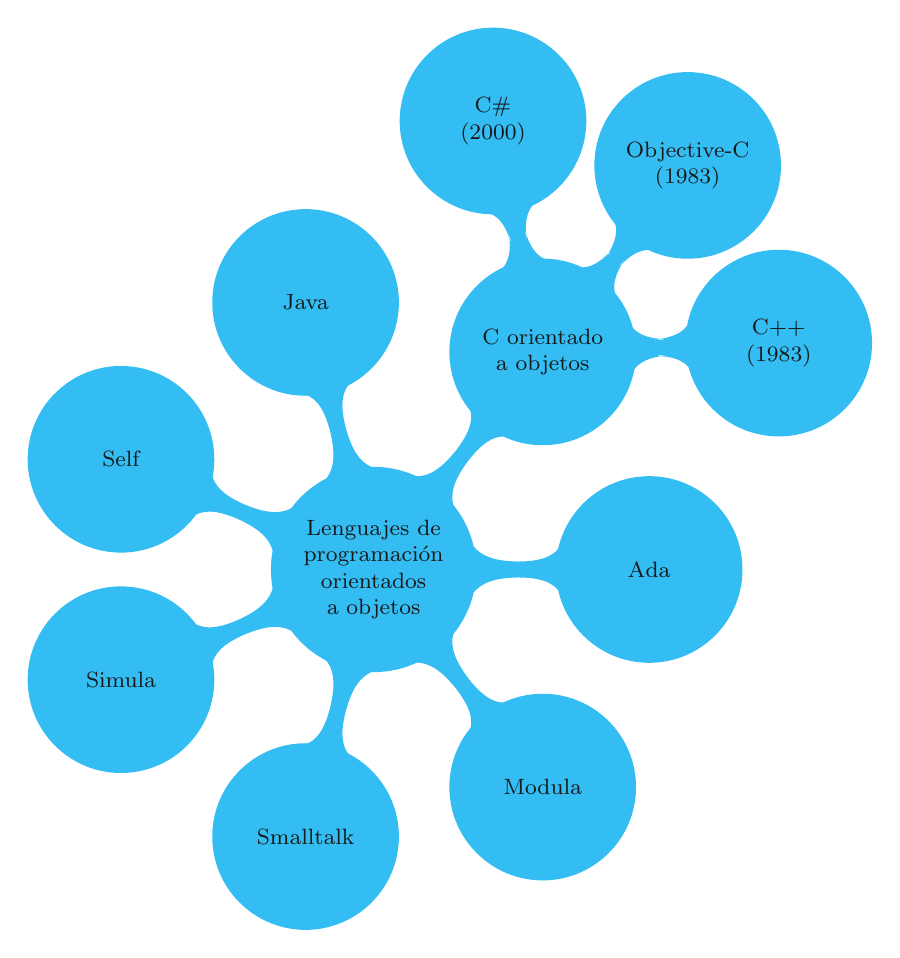
\begin{tikzpicture}[small mindmap, grow cyclic, every node/.style=concept, concept color=cyan!80, text=black!90,
    level 1/.style={level distance=3.5cm,sibling angle=365/7},
    level 2/.style={level distance=3cm,sibling angle=50},
    level 3/.style={level distance=3cm,sibling angle=20}]
    \node { Lenguajes de programación orientados a objetos}
    child { node { Simula } }
    child { node { Smalltalk } }
    child { node { Modula } }
    child { node { Ada } }
    child { node { C orientado a objetos }
        child { node { C++\\(1983)} }
        child { node { Objective-C\\(1983)} }
        child { node { C\#\\(2000)} }
    }
    child { node { Java } }
    child { node { Self } }
    ;
\end{tikzpicture}
\end{center}
\end{document}

